\documentclass[11pt]{article}

% Preamble

\usepackage[margin=1in]{geometry}
\usepackage{amsfonts, amsmath, amssymb}
\usepackage{fancyhdr, float, graphicx}
\usepackage[utf8]{inputenc} % Required for inputting international characters
\usepackage[T1]{fontenc} % Output font encoding for international characters
\usepackage{fouriernc} % Use the New Century Schoolbook font
\usepackage[nottoc, notlot, notlof]{tocbibind}
\usepackage{listings}
\usepackage{xcolor}
\usepackage{karnaugh-map}
% \usepackage[table,xcdraw]{xcolor}

\definecolor{codegreen}{rgb}{0,0.6,0}
\definecolor{codegray}{rgb}{0.5,0.5,0.5}
\definecolor{codepurple}{rgb}{0.58,0,0.82}
\definecolor{backcolour}{rgb}{0.95,0.95,0.92}

\lstdefinestyle{mystyle}{
    backgroundcolor=\color{backcolour},   
    commentstyle=\color{codegreen},
    keywordstyle=\color{magenta},
    numberstyle=\tiny\color{codegray},
    stringstyle=\color{codepurple},
    basicstyle=\ttfamily\footnotesize,
    breakatwhitespace=false,         
    breaklines=true,                 
    captionpos=b,                    
    keepspaces=true,                 
    numbers=left,                    
    numbersep=5pt,                  
    showspaces=false,                
    showstringspaces=false,
    showtabs=false,                  
    tabsize=2
}

\lstset{style=mystyle}

% Header and Footer
\pagestyle{fancy}
\fancyhead{}
\fancyfoot{}
\fancyhead[L]{\textit{\Large{DECA Assignment 6}}}
%\fancyhead[R]{\textit{something}}
\fancyfoot[C]{\thepage}
\renewcommand{\footrulewidth}{1pt}



% Other Doc Editing
% \parindent 0ex
%\renewcommand{\baselinestretch}{1.5}

\begin{document}

\begin{titlepage}
	\centering

	%---------------------------NAMES-------------------------------

	\huge\textsc{
		MIT World Peace University
	}\\

	\vspace{0.75\baselineskip} % space after Uni Name

	\LARGE{
		Digital Electronics and Computer Architecture\\
		Second Year B. Tech, Semester 3
	}

	\vfill % space after Sub Name

	%--------------------------TITLE-------------------------------

	\rule{\textwidth}{1.6pt}\vspace*{-\baselineskip}\vspace*{2pt}
	\rule{\textwidth}{0.6pt}
	\vspace{0.75\baselineskip} % Whitespace above the title



	\huge{\textsc{
			Design a sequence detector to detect the bit sequence 110 using Mealy Machine.
		}} \\



	\vspace{0.5\baselineskip} % Whitespace below the title
	\rule{\textwidth}{0.6pt}\vspace*{-\baselineskip}\vspace*{2.8pt}
	\rule{\textwidth}{1.6pt}

	\vspace{1\baselineskip} % Whitespace after the title block

	%--------------------------SUBTITLE --------------------------	

	\LARGE\textsc{
		Practical Report\\
		Assignment 6
	} % Subtitle or further description
	\vfill

	%--------------------------AUTHOR-------------------------------

	\vspace{0.5\baselineskip} % Whitespace before the editors

	\Large{
		Krishnaraj Thadesar \\
		Cyber Security and Forensics\\
		Batch A1, PA 20
	}


	\vspace{0.5\baselineskip} % Whitespace below the editor list
	\today

\end{titlepage}


\tableofcontents
\thispagestyle{empty}
\clearpage


\setcounter{page}{1}
\section{Objectives}
\begin{enumerate}
	\item To learn Finite State Machine
	\item To understand Moore and Mealy Machine
	\item To learn and implement Sequence Detector


\end{enumerate}

\section{Problem Statement}
Design a sequence detector to detect the bit sequence 110 using Mealy Machine.


\section{ICs Used}

\begin{enumerate}
	\item IC7408 (AND Gate)
	\item IC7476 (Dual Master Slave JK Flip Flop)
\end{enumerate}

\section{Platform Used}
Digital Trainer Kit

\section{Theory}
\subsection{Application of state machine}

A state machine is any device storing the status of something at a given time. The status changes based on inputs, providing the resulting output for the implemented changes. A finite state machine has finite internal memory.\\

They are used in applications where distinguishable sates exist. Each state can lead to one or multiple states and can also end the process flow. A state machine relies on user input and its original state calculation to determine to which state to go to next.

\subsection{Comparison Mealy Machine with Moore Machine}
\subsubsection{Mealy Machine}
\begin{enumerate}
	\item Output depends on the present state as well as present input.
	\item Mealy machine places its output on transition.
	\item Less number of states are required.
	\item Asynchronous output generation.
\end{enumerate}

\subsubsection{Moore Machine}
\begin{enumerate}
	\item Output depends only upon the present state.
	\item Moore machine also places its outputs on transition.
	\item Moore states are required.
	\item Synchronous output and state generation.
\end{enumerate}
\subsubsection{Sequence detector circuit}

A sequence detector is a sequential circuit that outputs certain data when a particular pattern of bits sequencitally arrives at its data input.

\subsection{Involved Truth Tables}

\subsubsection{AND Gate}

\begin{table}[H]
	\begin{tabular}{|c|c|c|}
		\hline
		{\color[HTML]{000000} \textbf{A}} & {\color[HTML]{000000} \textbf{B}} & {\color[HTML]{000000} \textbf{Q}} \\ \hline
		{\color[HTML]{330001} \textit{0}} & {\color[HTML]{330001} \textit{0}} & {\color[HTML]{F56B00} \textit{0}} \\ \hline
		{\color[HTML]{330001} \textit{0}} & {\color[HTML]{330001} \textit{1}} & {\color[HTML]{F56B00} \textit{1}} \\ \hline
		{\color[HTML]{330001} \textit{1}} & {\color[HTML]{330001} \textit{0}} & {\color[HTML]{F56B00} \textit{1}} \\ \hline
		{\color[HTML]{330001} \textit{1}} & {\color[HTML]{330001} \textit{1}} & {\color[HTML]{F56B00} \textit{1}} \\ \hline
	\end{tabular}
\end{table}

\subsubsection{Function Table of the IC7476}
\begin{figure}[H]
	\centering
	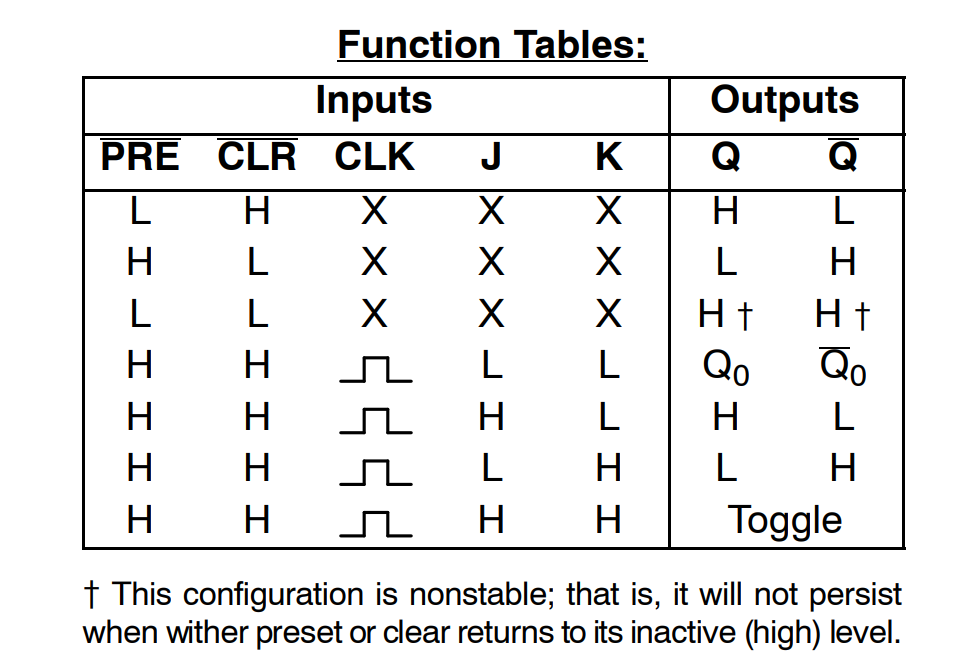
\includegraphics[scale = 0.5]{7476 function table.png}
	\caption{Function Table for IC 7476}
\end{figure}

\section{Pin Diagrams of ICs Used}

\subsection{Pin Diagram of IC7476}
\begin{figure}[H]
	\centering
	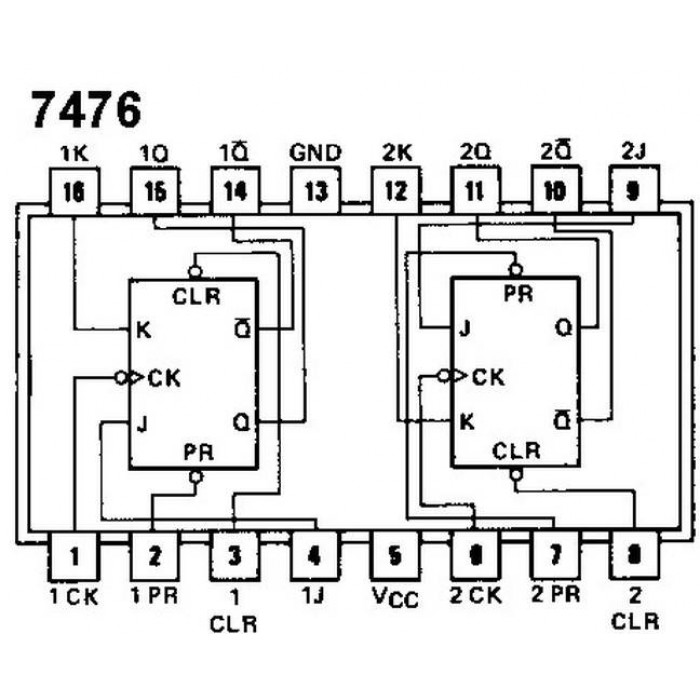
\includegraphics[scale = 0.35]{7476.jpg}
	\caption{Pin Diagram for IC 7476}
\end{figure}
\subsection{Pin Diagram of IC7408}
\begin{figure}[H]
	\centering
	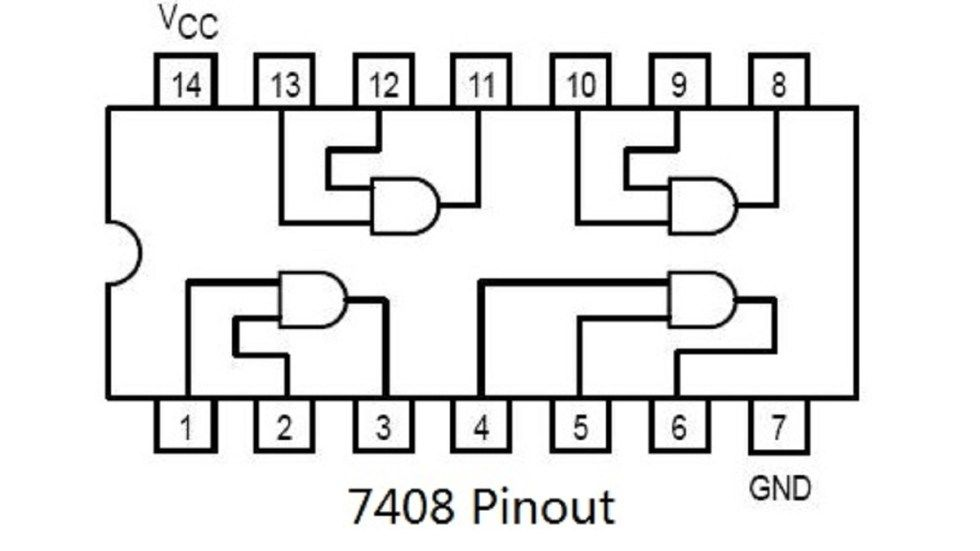
\includegraphics[scale = 0.25]{7408.jpg}
	\caption{Pin Diagram for IC 7408}
\end{figure}

\section{Design and Implementation}

\subsection{State Diagram}
\begin{figure}[H]
	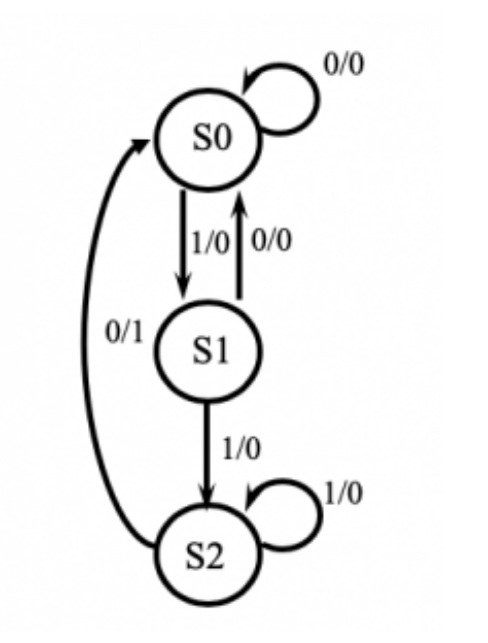
\includegraphics[width=0.45\textwidth]{state diagram.png}
	\caption{State Diagram}
	\label{fig:}
\end{figure}


\subsection{State Transition Table}
\begin{table}[H]
	\begin{tabular}{|ll|lll|llll|l|}
		\hline
		\multicolumn{2}{|l|}{\textbf{Present State}} & \multicolumn{3}{l|}{\textbf{Input Next State}} & \multicolumn{4}{l|}{\textbf{Flip Flop Input}} & \textbf{Output}                                                                                                                                                                         \\ \hline
		\multicolumn{1}{|l|}{\textbf{Qa}}            & \textbf{Qb}                                    & \multicolumn{1}{l|}{\textbf{X}}               & \multicolumn{1}{l|}{\textbf{Qa+1}} & \textbf{Qb+ 1} & \multicolumn{1}{l|}{\textbf{Ja}} & \multicolumn{1}{l|}{\textbf{Ka}} & \multicolumn{1}{l|}{\textbf{Jb}} & \textbf{Kb} & \textbf{Y} \\ \hline
		\multicolumn{1}{|l|}{0}                      & 0                                              & \multicolumn{1}{l|}{0}                        & \multicolumn{1}{l|}{0}             & 0              & \multicolumn{1}{l|}{0}           & \multicolumn{1}{l|}{X}           & \multicolumn{1}{l|}{0}           & X           & 0          \\ \hline
		\multicolumn{1}{|l|}{0}                      & 0                                              & \multicolumn{1}{l|}{1}                        & \multicolumn{1}{l|}{0}             & 1              & \multicolumn{1}{l|}{0}           & \multicolumn{1}{l|}{x}           & \multicolumn{1}{l|}{1}           & x           & 0          \\ \hline
		\multicolumn{1}{|l|}{0}                      & 1                                              & \multicolumn{1}{l|}{0}                        & \multicolumn{1}{l|}{0}             & 0              & \multicolumn{1}{l|}{0}           & \multicolumn{1}{l|}{x}           & \multicolumn{1}{l|}{x}           & 1           & 0          \\ \hline
		\multicolumn{1}{|l|}{0}                      & 1                                              & \multicolumn{1}{l|}{1}                        & \multicolumn{1}{l|}{1}             & 0              & \multicolumn{1}{l|}{1}           & \multicolumn{1}{l|}{x}           & \multicolumn{1}{l|}{x}           & 1           & 0          \\ \hline
		\multicolumn{1}{|l|}{1}                      & 0                                              & \multicolumn{1}{l|}{0}                        & \multicolumn{1}{l|}{0}             & 0              & \multicolumn{1}{l|}{x}           & \multicolumn{1}{l|}{1}           & \multicolumn{1}{l|}{0}           & x           & 1          \\ \hline
		\multicolumn{1}{|l|}{1}                      & 0                                              & \multicolumn{1}{l|}{1}                        & \multicolumn{1}{l|}{0}             & 1              & \multicolumn{1}{l|}{x}           & \multicolumn{1}{l|}{1}           & \multicolumn{1}{l|}{1}           & x           & 0          \\ \hline
		\multicolumn{1}{|l|}{1}                      & 1                                              & \multicolumn{1}{l|}{0}                        & \multicolumn{1}{l|}{x}             & x              & \multicolumn{1}{l|}{x}           & \multicolumn{1}{l|}{x}           & \multicolumn{1}{l|}{x}           & x           & x          \\ \hline
		\multicolumn{1}{|l|}{1}                      & 1                                              & \multicolumn{1}{l|}{1}                        & \multicolumn{1}{l|}{x}             & x              & \multicolumn{1}{l|}{x}           & \multicolumn{1}{l|}{x}           & \multicolumn{1}{l|}{x}           & x           & x          \\ \hline
	\end{tabular}
\end{table}


\subsection{State Assignment}
\textbf{A = 00}
\textbf{B = 01}
\textbf{C = 10}

\section{K-Maps}

\begin{karnaugh-map}[4][2][1][$Q_{A}$][$Q_{B}$][$1$]
\manualterms{0, 0, 0, 1, X, X, X, X}
% \autoterms[0]
% \implicant{3}{3}
\end{karnaugh-map}

\[J_A = Q_{a + 1}X\]
\begin{karnaugh-map}[4][2][1][$Q_{A}$][$Q_{B}$][$1$]
	\manualterms{0, X, X, X, X, X, X, X}
% \autoterms[0]

\end{karnaugh-map}
\[K_A = 1\]

\begin{karnaugh-map}[4][2][1][$Q_{A}$][$Q_{B}$][$1$]
	\manualterms{0, 1, X, X, 0, 1, X, X}
% \autoterms[0]

\end{karnaugh-map}
\[J_B = X\]

\begin{karnaugh-map}[4][2][1][$Q_{A}$][$Q_{B}$][$1$]
	\manualterms{X, X, X, X, X, X, X, X}
% \autoterms[0]

\end{karnaugh-map}

\[K_B = 1\]

\begin{karnaugh-map}[4][2][1][$Q_{A}$][$Q_{B}$][$1$]
	\manualterms{0, 0, 0, 0, 1, 0, X, X}
% \autoterms[0]

\end{karnaugh-map}
\[Y=Q_a \Bar{X}\]


\section{Circuit Diagram}
\begin{figure}[H]
	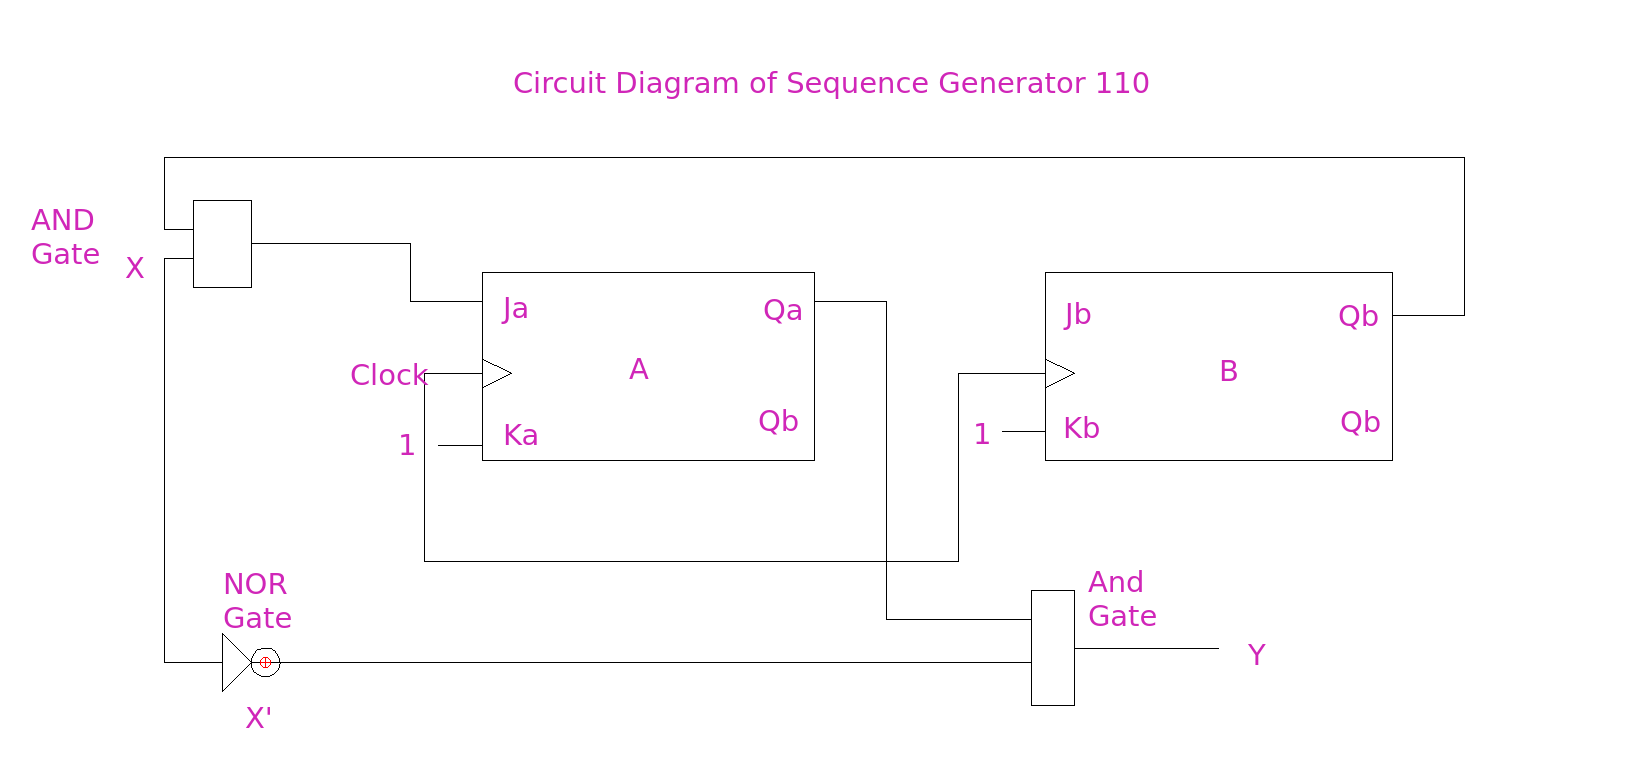
\includegraphics[scale=0.4]{circuit diagram for sg.png}
	\label{fig:}
\end{figure}



\section{Procedure}

\begin{enumerate}
	\item Draw state diagram
	\item Make a state table
	\item Apply state reduction if required
	\item Assign states
	\item Re-write the state table using states assigned
	\item Prepare state transition table
	\item Use k-maps to find inputs to Flip Flop
	\item Draw the circuit diagram.
\end{enumerate}

\section{Conclusion}
\textit{Thus, we have learnt a about Working of Mealy Machines. State diagrams, transition diagrams and conversion of K-maps to Boolean expressions were also studied. We have also learnt how to design a Mealy Machine using the above mentioned concepts.}
\pagebreak

\section{FAQs}

\begin{enumerate}
	\item What is Sequence Detector?

	      A sequence detector is a sequential circuit that outputs 1 when a particular pattern of bits sequentially arrives at its data input. The figure below shows a block diagram of a sequence detector. It has two inputs and one output. The inputs are the clock used to synchronize the functionality of the circuit and the data input.

	      Sequence detector is of two types:
	      \begin{itemize}
		      \item Overlapping
		      \item Non-Overlapping
	      \end{itemize}

	      In an overlapping sequence detector, the last bit of one sequence becomes the first bit of the next sequence. However, in a non-overlapping sequence detector, the last bit of one sequence does not become the first bit of the next sequence. In this post, we'll discuss the design procedure for non-overlapping 101 Mealy sequence detectors.

	\item What are applications of Sequence Detector?

	      \begin{itemize}
		      \item Sequence detectors are used in the decoding equipment on the ground to provide “flags” which indicate the beginning (or end) of a data block (e.g., a TV frame).
		      \item They can be used to detect if a bunch of states in a circuit occur in a particular desired pattern.

	      \end{itemize}

\end{enumerate}

\end{document}